\documentclass[margin=2mm]{standalone}
\usepackage{tikz}
\usepackage{amsmath,amssymb,mathtools}
\begin{document}
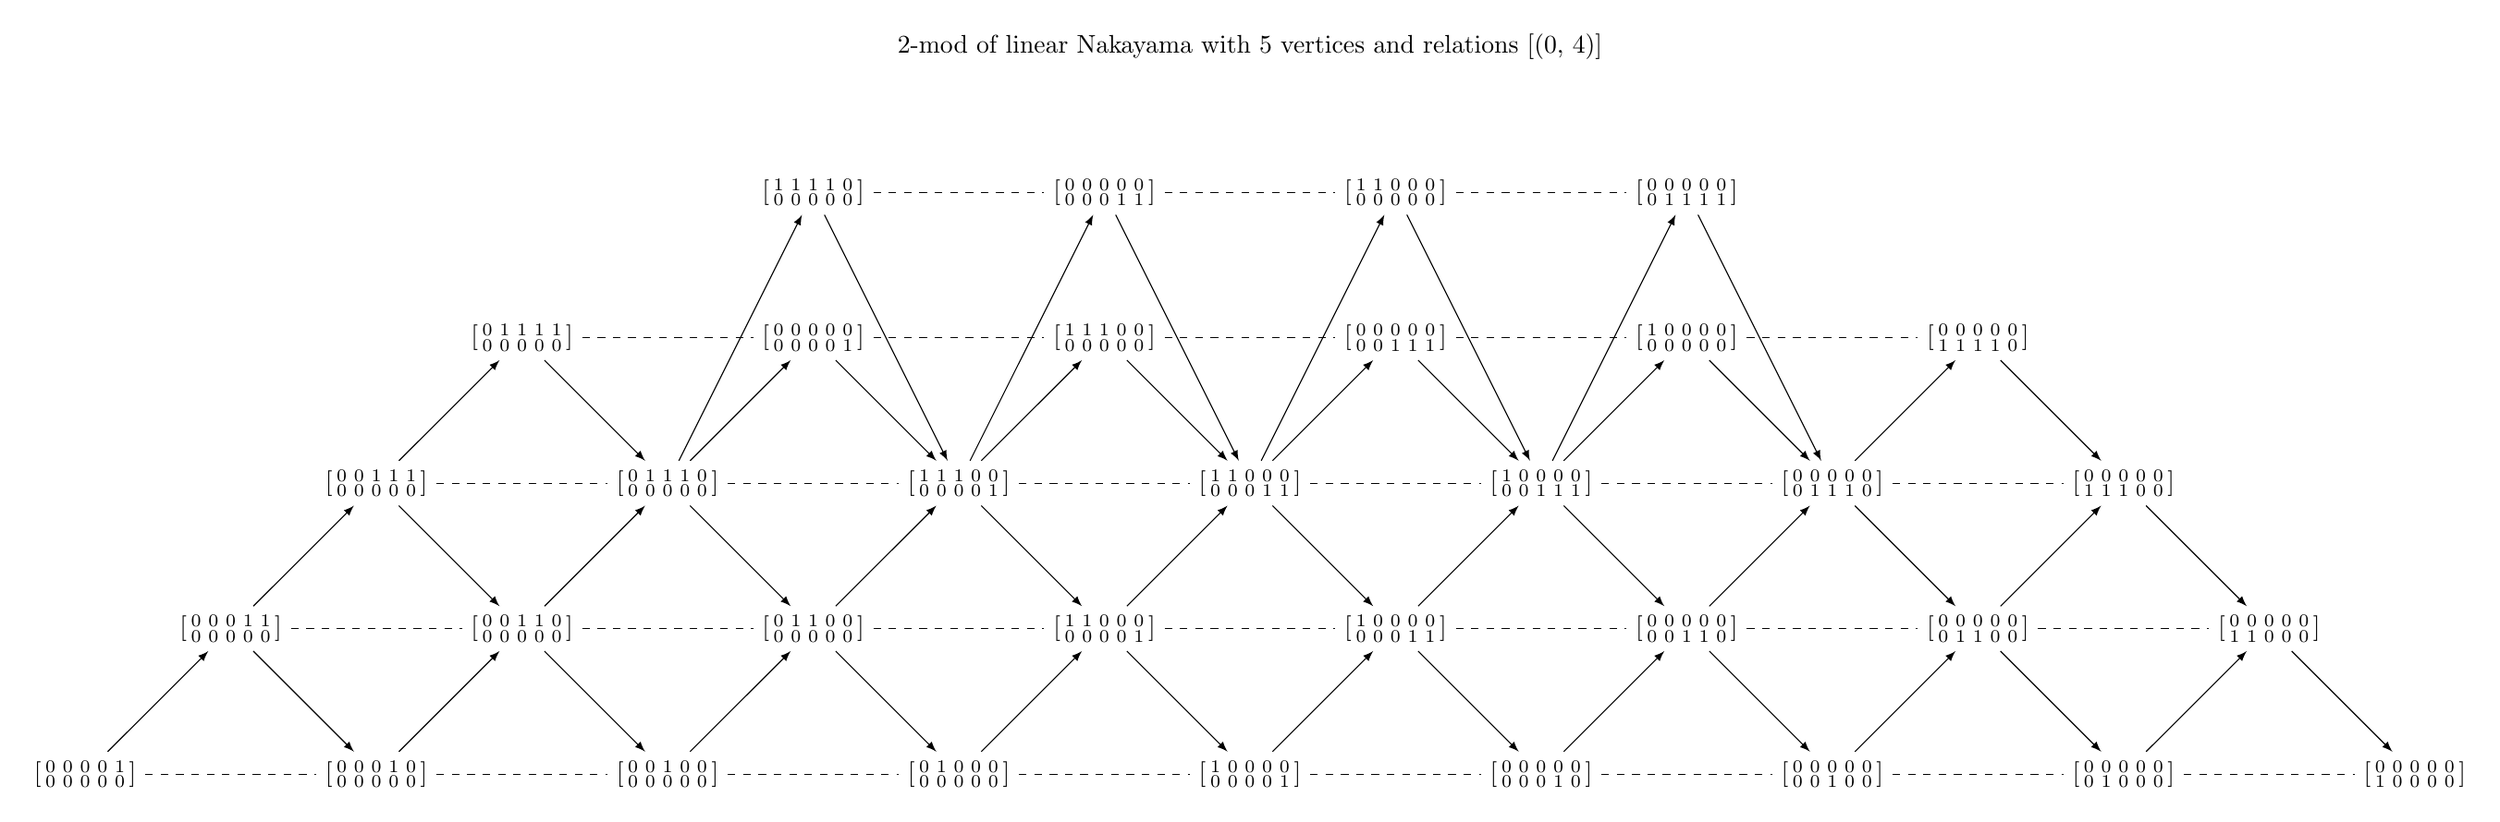
\begin{tikzpicture}[xscale=2,yscale=2]
\node at (8.0,5) [] {$2$-mod of linear Nakayama with 5 vertices and relations [(0, 4)]};
\node (t-0P0) at (5,4) [scale=1] {$\begin{bsmallmatrix}
 1 & 1 & 1 & 1 & 0\\
 0 & 0 & 0 & 0 & 0\\
\end{bsmallmatrix}$};
\node (t-1P0) at (7,4) [scale=1] {$\begin{bsmallmatrix}
 0 & 0 & 0 & 0 & 0\\
 0 & 0 & 0 & 1 & 1\\
\end{bsmallmatrix}$};
\node (t-2P0) at (9,4) [scale=1] {$\begin{bsmallmatrix}
 1 & 1 & 0 & 0 & 0\\
 0 & 0 & 0 & 0 & 0\\
\end{bsmallmatrix}$};
\node (t-3P0) at (11,4) [scale=1] {$\begin{bsmallmatrix}
 0 & 0 & 0 & 0 & 0\\
 0 & 1 & 1 & 1 & 1\\
\end{bsmallmatrix}$};
\node (t-0P1) at (3,3) [scale=1] {$\begin{bsmallmatrix}
 0 & 1 & 1 & 1 & 1\\
 0 & 0 & 0 & 0 & 0\\
\end{bsmallmatrix}$};
\node (t-1P1) at (5,3) [scale=1] {$\begin{bsmallmatrix}
 0 & 0 & 0 & 0 & 0\\
 0 & 0 & 0 & 0 & 1\\
\end{bsmallmatrix}$};
\node (t-2P1) at (7,3) [scale=1] {$\begin{bsmallmatrix}
 1 & 1 & 1 & 0 & 0\\
 0 & 0 & 0 & 0 & 0\\
\end{bsmallmatrix}$};
\node (t-3P1) at (9,3) [scale=1] {$\begin{bsmallmatrix}
 0 & 0 & 0 & 0 & 0\\
 0 & 0 & 1 & 1 & 1\\
\end{bsmallmatrix}$};
\node (t-4P1) at (11,3) [scale=1] {$\begin{bsmallmatrix}
 1 & 0 & 0 & 0 & 0\\
 0 & 0 & 0 & 0 & 0\\
\end{bsmallmatrix}$};
\node (t-5P1) at (13,3) [scale=1] {$\begin{bsmallmatrix}
 0 & 0 & 0 & 0 & 0\\
 1 & 1 & 1 & 1 & 0\\
\end{bsmallmatrix}$};
\node (t-0P2) at (2,2) [scale=1] {$\begin{bsmallmatrix}
 0 & 0 & 1 & 1 & 1\\
 0 & 0 & 0 & 0 & 0\\
\end{bsmallmatrix}$};
\node (t-1P2) at (4,2) [scale=1] {$\begin{bsmallmatrix}
 0 & 1 & 1 & 1 & 0\\
 0 & 0 & 0 & 0 & 0\\
\end{bsmallmatrix}$};
\node (t-2P2) at (6,2) [scale=1] {$\begin{bsmallmatrix}
 1 & 1 & 1 & 0 & 0\\
 0 & 0 & 0 & 0 & 1\\
\end{bsmallmatrix}$};
\node (t-3P2) at (8,2) [scale=1] {$\begin{bsmallmatrix}
 1 & 1 & 0 & 0 & 0\\
 0 & 0 & 0 & 1 & 1\\
\end{bsmallmatrix}$};
\node (t-4P2) at (10,2) [scale=1] {$\begin{bsmallmatrix}
 1 & 0 & 0 & 0 & 0\\
 0 & 0 & 1 & 1 & 1\\
\end{bsmallmatrix}$};
\node (t-5P2) at (12,2) [scale=1] {$\begin{bsmallmatrix}
 0 & 0 & 0 & 0 & 0\\
 0 & 1 & 1 & 1 & 0\\
\end{bsmallmatrix}$};
\node (t-6P2) at (14,2) [scale=1] {$\begin{bsmallmatrix}
 0 & 0 & 0 & 0 & 0\\
 1 & 1 & 1 & 0 & 0\\
\end{bsmallmatrix}$};
\node (t-0P3) at (1,1) [scale=1] {$\begin{bsmallmatrix}
 0 & 0 & 0 & 1 & 1\\
 0 & 0 & 0 & 0 & 0\\
\end{bsmallmatrix}$};
\node (t-1P3) at (3,1) [scale=1] {$\begin{bsmallmatrix}
 0 & 0 & 1 & 1 & 0\\
 0 & 0 & 0 & 0 & 0\\
\end{bsmallmatrix}$};
\node (t-2P3) at (5,1) [scale=1] {$\begin{bsmallmatrix}
 0 & 1 & 1 & 0 & 0\\
 0 & 0 & 0 & 0 & 0\\
\end{bsmallmatrix}$};
\node (t-3P3) at (7,1) [scale=1] {$\begin{bsmallmatrix}
 1 & 1 & 0 & 0 & 0\\
 0 & 0 & 0 & 0 & 1\\
\end{bsmallmatrix}$};
\node (t-4P3) at (9,1) [scale=1] {$\begin{bsmallmatrix}
 1 & 0 & 0 & 0 & 0\\
 0 & 0 & 0 & 1 & 1\\
\end{bsmallmatrix}$};
\node (t-5P3) at (11,1) [scale=1] {$\begin{bsmallmatrix}
 0 & 0 & 0 & 0 & 0\\
 0 & 0 & 1 & 1 & 0\\
\end{bsmallmatrix}$};
\node (t-6P3) at (13,1) [scale=1] {$\begin{bsmallmatrix}
 0 & 0 & 0 & 0 & 0\\
 0 & 1 & 1 & 0 & 0\\
\end{bsmallmatrix}$};
\node (t-7P3) at (15,1) [scale=1] {$\begin{bsmallmatrix}
 0 & 0 & 0 & 0 & 0\\
 1 & 1 & 0 & 0 & 0\\
\end{bsmallmatrix}$};
\node (t-0P4) at (0,0) [scale=1] {$\begin{bsmallmatrix}
 0 & 0 & 0 & 0 & 1\\
 0 & 0 & 0 & 0 & 0\\
\end{bsmallmatrix}$};
\node (t-1P4) at (2,0) [scale=1] {$\begin{bsmallmatrix}
 0 & 0 & 0 & 1 & 0\\
 0 & 0 & 0 & 0 & 0\\
\end{bsmallmatrix}$};
\node (t-2P4) at (4,0) [scale=1] {$\begin{bsmallmatrix}
 0 & 0 & 1 & 0 & 0\\
 0 & 0 & 0 & 0 & 0\\
\end{bsmallmatrix}$};
\node (t-3P4) at (6,0) [scale=1] {$\begin{bsmallmatrix}
 0 & 1 & 0 & 0 & 0\\
 0 & 0 & 0 & 0 & 0\\
\end{bsmallmatrix}$};
\node (t-4P4) at (8,0) [scale=1] {$\begin{bsmallmatrix}
 1 & 0 & 0 & 0 & 0\\
 0 & 0 & 0 & 0 & 1\\
\end{bsmallmatrix}$};
\node (t-5P4) at (10,0) [scale=1] {$\begin{bsmallmatrix}
 0 & 0 & 0 & 0 & 0\\
 0 & 0 & 0 & 1 & 0\\
\end{bsmallmatrix}$};
\node (t-6P4) at (12,0) [scale=1] {$\begin{bsmallmatrix}
 0 & 0 & 0 & 0 & 0\\
 0 & 0 & 1 & 0 & 0\\
\end{bsmallmatrix}$};
\node (t-7P4) at (14,0) [scale=1] {$\begin{bsmallmatrix}
 0 & 0 & 0 & 0 & 0\\
 0 & 1 & 0 & 0 & 0\\
\end{bsmallmatrix}$};
\node (t-8P4) at (16,0) [scale=1] {$\begin{bsmallmatrix}
 0 & 0 & 0 & 0 & 0\\
 1 & 0 & 0 & 0 & 0\\
\end{bsmallmatrix}$};
\draw[-latex] (t-0P0) -- (t-2P2);
\draw[-latex] (t-1P0) -- (t-3P2);
\draw[-latex] (t-2P0) -- (t-4P2);
\draw[-latex] (t-3P0) -- (t-5P2);
\draw[-latex] (t-0P1) -- (t-1P2);
\draw[-latex] (t-1P1) -- (t-2P2);
\draw[-latex] (t-2P1) -- (t-3P2);
\draw[-latex] (t-3P1) -- (t-4P2);
\draw[-latex] (t-4P1) -- (t-5P2);
\draw[-latex] (t-5P1) -- (t-6P2);
\draw[-latex] (t-0P2) -- (t-0P1);
\draw[-latex] (t-0P2) -- (t-1P3);
\draw[-latex] (t-1P2) -- (t-0P0);
\draw[-latex] (t-1P2) -- (t-1P1);
\draw[-latex] (t-1P2) -- (t-2P3);
\draw[-latex] (t-2P2) -- (t-1P0);
\draw[-latex] (t-2P2) -- (t-2P1);
\draw[-latex] (t-2P2) -- (t-3P3);
\draw[-latex] (t-3P2) -- (t-2P0);
\draw[-latex] (t-3P2) -- (t-3P1);
\draw[-latex] (t-3P2) -- (t-4P3);
\draw[-latex] (t-4P2) -- (t-3P0);
\draw[-latex] (t-4P2) -- (t-4P1);
\draw[-latex] (t-4P2) -- (t-5P3);
\draw[-latex] (t-5P2) -- (t-5P1);
\draw[-latex] (t-5P2) -- (t-6P3);
\draw[-latex] (t-6P2) -- (t-7P3);
\draw[-latex] (t-0P3) -- (t-0P2);
\draw[-latex] (t-0P3) -- (t-1P4);
\draw[-latex] (t-1P3) -- (t-1P2);
\draw[-latex] (t-1P3) -- (t-2P4);
\draw[-latex] (t-2P3) -- (t-2P2);
\draw[-latex] (t-2P3) -- (t-3P4);
\draw[-latex] (t-3P3) -- (t-3P2);
\draw[-latex] (t-3P3) -- (t-4P4);
\draw[-latex] (t-4P3) -- (t-4P2);
\draw[-latex] (t-4P3) -- (t-5P4);
\draw[-latex] (t-5P3) -- (t-5P2);
\draw[-latex] (t-5P3) -- (t-6P4);
\draw[-latex] (t-6P3) -- (t-6P2);
\draw[-latex] (t-6P3) -- (t-7P4);
\draw[-latex] (t-7P3) -- (t-8P4);
\draw[-latex] (t-0P4) -- (t-0P3);
\draw[-latex] (t-1P4) -- (t-1P3);
\draw[-latex] (t-2P4) -- (t-2P3);
\draw[-latex] (t-3P4) -- (t-3P3);
\draw[-latex] (t-4P4) -- (t-4P3);
\draw[-latex] (t-5P4) -- (t-5P3);
\draw[-latex] (t-6P4) -- (t-6P3);
\draw[-latex] (t-7P4) -- (t-7P3);
\draw[dashed] (t-0P0)--(t-1P0);
\draw[dashed] (t-1P0)--(t-2P0);
\draw[dashed] (t-2P0)--(t-3P0);
\draw[dashed] (t-0P1)--(t-1P1);
\draw[dashed] (t-1P1)--(t-2P1);
\draw[dashed] (t-2P1)--(t-3P1);
\draw[dashed] (t-3P1)--(t-4P1);
\draw[dashed] (t-4P1)--(t-5P1);
\draw[dashed] (t-0P2)--(t-1P2);
\draw[dashed] (t-1P2)--(t-2P2);
\draw[dashed] (t-2P2)--(t-3P2);
\draw[dashed] (t-3P2)--(t-4P2);
\draw[dashed] (t-4P2)--(t-5P2);
\draw[dashed] (t-5P2)--(t-6P2);
\draw[dashed] (t-0P3)--(t-1P3);
\draw[dashed] (t-1P3)--(t-2P3);
\draw[dashed] (t-2P3)--(t-3P3);
\draw[dashed] (t-3P3)--(t-4P3);
\draw[dashed] (t-4P3)--(t-5P3);
\draw[dashed] (t-5P3)--(t-6P3);
\draw[dashed] (t-6P3)--(t-7P3);
\draw[dashed] (t-0P4)--(t-1P4);
\draw[dashed] (t-1P4)--(t-2P4);
\draw[dashed] (t-2P4)--(t-3P4);
\draw[dashed] (t-3P4)--(t-4P4);
\draw[dashed] (t-4P4)--(t-5P4);
\draw[dashed] (t-5P4)--(t-6P4);
\draw[dashed] (t-6P4)--(t-7P4);
\draw[dashed] (t-7P4)--(t-8P4);
\end{tikzpicture}\end{document}